\documentclass[]{article}
\usepackage{lmodern}
\usepackage{amssymb,amsmath}
\usepackage{ifxetex,ifluatex}
\usepackage{fixltx2e} % provides \textsubscript
\ifnum 0\ifxetex 1\fi\ifluatex 1\fi=0 % if pdftex
  \usepackage[T1]{fontenc}
  \usepackage[utf8]{inputenc}
\else % if luatex or xelatex
  \ifxetex
    \usepackage{mathspec}
  \else
    \usepackage{fontspec}
  \fi
  \defaultfontfeatures{Ligatures=TeX,Scale=MatchLowercase}
\fi
% use upquote if available, for straight quotes in verbatim environments
\IfFileExists{upquote.sty}{\usepackage{upquote}}{}
% use microtype if available
\IfFileExists{microtype.sty}{%
\usepackage{microtype}
\UseMicrotypeSet[protrusion]{basicmath} % disable protrusion for tt fonts
}{}
\usepackage[margin=1in]{geometry}
\usepackage{hyperref}
\hypersetup{unicode=true,
            pdftitle={BSc Coursework 2},
            pdfauthor={Salik Tariq / Student ID: 12516369},
            pdfborder={0 0 0},
            breaklinks=true}
\urlstyle{same}  % don't use monospace font for urls
\usepackage{color}
\usepackage{fancyvrb}
\newcommand{\VerbBar}{|}
\newcommand{\VERB}{\Verb[commandchars=\\\{\}]}
\DefineVerbatimEnvironment{Highlighting}{Verbatim}{commandchars=\\\{\}}
% Add ',fontsize=\small' for more characters per line
\usepackage{framed}
\definecolor{shadecolor}{RGB}{248,248,248}
\newenvironment{Shaded}{\begin{snugshade}}{\end{snugshade}}
\newcommand{\AlertTok}[1]{\textcolor[rgb]{0.94,0.16,0.16}{#1}}
\newcommand{\AnnotationTok}[1]{\textcolor[rgb]{0.56,0.35,0.01}{\textbf{\textit{#1}}}}
\newcommand{\AttributeTok}[1]{\textcolor[rgb]{0.77,0.63,0.00}{#1}}
\newcommand{\BaseNTok}[1]{\textcolor[rgb]{0.00,0.00,0.81}{#1}}
\newcommand{\BuiltInTok}[1]{#1}
\newcommand{\CharTok}[1]{\textcolor[rgb]{0.31,0.60,0.02}{#1}}
\newcommand{\CommentTok}[1]{\textcolor[rgb]{0.56,0.35,0.01}{\textit{#1}}}
\newcommand{\CommentVarTok}[1]{\textcolor[rgb]{0.56,0.35,0.01}{\textbf{\textit{#1}}}}
\newcommand{\ConstantTok}[1]{\textcolor[rgb]{0.00,0.00,0.00}{#1}}
\newcommand{\ControlFlowTok}[1]{\textcolor[rgb]{0.13,0.29,0.53}{\textbf{#1}}}
\newcommand{\DataTypeTok}[1]{\textcolor[rgb]{0.13,0.29,0.53}{#1}}
\newcommand{\DecValTok}[1]{\textcolor[rgb]{0.00,0.00,0.81}{#1}}
\newcommand{\DocumentationTok}[1]{\textcolor[rgb]{0.56,0.35,0.01}{\textbf{\textit{#1}}}}
\newcommand{\ErrorTok}[1]{\textcolor[rgb]{0.64,0.00,0.00}{\textbf{#1}}}
\newcommand{\ExtensionTok}[1]{#1}
\newcommand{\FloatTok}[1]{\textcolor[rgb]{0.00,0.00,0.81}{#1}}
\newcommand{\FunctionTok}[1]{\textcolor[rgb]{0.00,0.00,0.00}{#1}}
\newcommand{\ImportTok}[1]{#1}
\newcommand{\InformationTok}[1]{\textcolor[rgb]{0.56,0.35,0.01}{\textbf{\textit{#1}}}}
\newcommand{\KeywordTok}[1]{\textcolor[rgb]{0.13,0.29,0.53}{\textbf{#1}}}
\newcommand{\NormalTok}[1]{#1}
\newcommand{\OperatorTok}[1]{\textcolor[rgb]{0.81,0.36,0.00}{\textbf{#1}}}
\newcommand{\OtherTok}[1]{\textcolor[rgb]{0.56,0.35,0.01}{#1}}
\newcommand{\PreprocessorTok}[1]{\textcolor[rgb]{0.56,0.35,0.01}{\textit{#1}}}
\newcommand{\RegionMarkerTok}[1]{#1}
\newcommand{\SpecialCharTok}[1]{\textcolor[rgb]{0.00,0.00,0.00}{#1}}
\newcommand{\SpecialStringTok}[1]{\textcolor[rgb]{0.31,0.60,0.02}{#1}}
\newcommand{\StringTok}[1]{\textcolor[rgb]{0.31,0.60,0.02}{#1}}
\newcommand{\VariableTok}[1]{\textcolor[rgb]{0.00,0.00,0.00}{#1}}
\newcommand{\VerbatimStringTok}[1]{\textcolor[rgb]{0.31,0.60,0.02}{#1}}
\newcommand{\WarningTok}[1]{\textcolor[rgb]{0.56,0.35,0.01}{\textbf{\textit{#1}}}}
\usepackage{graphicx,grffile}
\makeatletter
\def\maxwidth{\ifdim\Gin@nat@width>\linewidth\linewidth\else\Gin@nat@width\fi}
\def\maxheight{\ifdim\Gin@nat@height>\textheight\textheight\else\Gin@nat@height\fi}
\makeatother
% Scale images if necessary, so that they will not overflow the page
% margins by default, and it is still possible to overwrite the defaults
% using explicit options in \includegraphics[width, height, ...]{}
\setkeys{Gin}{width=\maxwidth,height=\maxheight,keepaspectratio}
\IfFileExists{parskip.sty}{%
\usepackage{parskip}
}{% else
\setlength{\parindent}{0pt}
\setlength{\parskip}{6pt plus 2pt minus 1pt}
}
\setlength{\emergencystretch}{3em}  % prevent overfull lines
\providecommand{\tightlist}{%
  \setlength{\itemsep}{0pt}\setlength{\parskip}{0pt}}
\setcounter{secnumdepth}{0}
% Redefines (sub)paragraphs to behave more like sections
\ifx\paragraph\undefined\else
\let\oldparagraph\paragraph
\renewcommand{\paragraph}[1]{\oldparagraph{#1}\mbox{}}
\fi
\ifx\subparagraph\undefined\else
\let\oldsubparagraph\subparagraph
\renewcommand{\subparagraph}[1]{\oldsubparagraph{#1}\mbox{}}
\fi

%%% Use protect on footnotes to avoid problems with footnotes in titles
\let\rmarkdownfootnote\footnote%
\def\footnote{\protect\rmarkdownfootnote}

%%% Change title format to be more compact
\usepackage{titling}

% Create subtitle command for use in maketitle
\providecommand{\subtitle}[1]{
  \posttitle{
    \begin{center}\large#1\end{center}
    }
}

\setlength{\droptitle}{-2em}

  \title{BSc Coursework 2}
    \pretitle{\vspace{\droptitle}\centering\huge}
  \posttitle{\par}
    \author{Salik Tariq / Student ID: 12516369}
    \preauthor{\centering\large\emph}
  \postauthor{\par}
    \date{}
    \predate{}\postdate{}
  

\begin{document}
\maketitle

\hypertarget{bayesian-networks-and-nauxefve-bayes-classifiers}{%
\section{1) Bayesian Networks and Naïve Bayes
Classifiers}\label{bayesian-networks-and-nauxefve-bayes-classifiers}}

\hypertarget{a-given-a-training-dataset-including-30-instances-and-a-bayesian-network-indicating-the-relationships-between-3-features-i.e.-income-student-and-credit-rate-and-the-class-attribute-i.e.-buy-computer-please-create-the-conditional-probability-tables-by-hand.}{%
\subsubsection{(a) Given a training dataset including 30 instances and a
Bayesian network indicating the relationships between 3 features
(i.e.~Income, Student and Credit Rate), and the class attribute
(i.e.~Buy Computer), please create the conditional probability tables by
hand.}\label{a-given-a-training-dataset-including-30-instances-and-a-bayesian-network-indicating-the-relationships-between-3-features-i.e.-income-student-and-credit-rate-and-the-class-attribute-i.e.-buy-computer-please-create-the-conditional-probability-tables-by-hand.}}

\hypertarget{student}{%
\subsection{Student}\label{student}}

\#\#Buy Computer \textbar{} True False
\#\#\_\_\_\_\_\_\_\_\_\_\_\_\_\_\_\_\_\_\_\_\_\_\_\_\_\_\_\_\_\_\_\_\_
\#\# YES \textbar{} 0.5 0.5 \#\# NO \textbar{} 0.6875 0.3125

\hypertarget{income}{%
\subsection{Income}\label{income}}

\#\#Buy Computer \textbar{} High Low
\#\#\_\_\_\_\_\_\_\_\_\_\_\_\_\_\_\_\_\_\_\_\_\_\_\_\_\_\_\_\_\_\_\_\_
\#\# YES \textbar{} 0.357 0.643 \#\# NO \textbar{} 0.4375 0.5625

\#\#Buy Computer\\
\#\#\_\_\_\_\_\_\_\_\_\_\_\_\_\_\_\_\_\_\_\_\_\_\_\_\_\_\_\_\_\_\_\_\_
\#\# YES \textbar{} 0.467 \#\# NO \textbar{} 0.533

\hypertarget{credit-rating}{%
\subsection{Credit Rating}\label{credit-rating}}

\#\#Income Student Buy Computer \textbar{} Fair Excellent
\#\#\_\_\_\_\_\_\_\_\_\_\_\_\_\_\_\_\_\_\_\_\_\_\_\_\_\_\_\_\_\_\_\_\_\_\textbar\_\_\_\_\_\_\_\_\_\_\_\_\_\_\_\_\_\_\_\_\_\_\_
\#\# High True Yes \textbar{} 0.5 0.5 \#\# Low True Yes \textbar{} 0.6
0.4 \#\# High False Yes \textbar{} 0.334 0.666 \#\# Low False Yes
\textbar{} 0.5 0.5 \#\# High True No \textbar{} 0.5 0.5 \#\# Low True No
\textbar{} 0.714 0.286 \#\# High False No \textbar{} 0.334 0.666 \#\#
Low False No \textbar{} 0.5 0.5

\hypertarget{b-make-predictions-for-2-testing-instances-by-using-the-bayesian-network-classifier}{%
\subsubsection{(b) Make predictions for 2 testing instances by using the
Bayesian network
classifier}\label{b-make-predictions-for-2-testing-instances-by-using-the-bayesian-network-classifier}}

Prediction for Instance\_31 Income = Low Student = False Credit Rating =
Excellent

To predict: Buy Computer?

P(Buy Computer=Yes, Income = Low, Student=False, Credit Rating =
Excellent) =P(Income=Low \textbar{} Buy Computer = Yes) \emph{P(Student
= False \textbar{} Buy Computer = Yes) }P(Credit Rating =
Excellent\textbar{} Income = Low, Student = False, Buy Computer = Yes)
*P(Buy Computer = Yes)

= 0.643 * 0.5 * 0.5 * 0.467 = 0.075

P(Buy Computer=No, Income = Low, Student=False, Credit Rating =
Excellent) =P(Income=Low \textbar{} Buy Computer = No) \emph{P(Student =
False \textbar{} Buy Computer = No) }P(Credit Rating =
Excellent\textbar{} Income = Low, Student = False, Buy Computer = No)
*P(Buy Computer = No)

= 0.5625 * 0.3125 * 0.5 * 0.533 = 0.0468

Prediction for Instance\_32 Income = High Student = False Credit Rating
= Fair

To predict: Buy Computer?

P(Buy Computer = Yes, Income = High, Student = False, Credit Rating =
Fair) =P(Income = High \textbar{} Buy Computer = Yes) \emph{P(Student =
False \textbar{} Buy Computer = Yes) }P(Credit Rating = Fair \textbar{}
Buy Computer = Yes, Student = False, Income = High) *P(Buy Computer =
Yes)

= 0.357 * 0.5 * 0.334 * 0.467 = 0.0278

P(Buy Computer = No, Income = High, Student = False, Credit Rating =
Fair) =P(Income = High \textbar{} Buy Computer = No) \emph{P(Student =
False \textbar{} Buy Computer = No) }P(Credit Rating = Fair \textbar{}
Buy Computer = No, Student = False, Income = High) *P(Buy Computer = No)

= 0.4375 * 0.3125 * 0.334 * 0.533 = 0.02434

\hypertarget{c-based-on-the-conditional-independence-assumption-between-features-please-create-the-conditional-probability-tables-by-hand.}{%
\subsubsection{(c) Based on the conditional independence assumption
between features, please create the conditional probability tables by
hand.}\label{c-based-on-the-conditional-independence-assumption-between-features-please-create-the-conditional-probability-tables-by-hand.}}

\hypertarget{student-1}{%
\subsection{Student}\label{student-1}}

\#\#Buy Computer \textbar{} True False
\#\#\_\_\_\_\_\_\_\_\_\_\_\_\_\_\_\_\_\_\_\_\_\_\_\_\_\_\_\_\_\_\_\_\_
\#\# YES \textbar{} 0.5 0.5 \#\# NO \textbar{} 0.6875 0.3125

\hypertarget{income-1}{%
\subsection{Income}\label{income-1}}

\#\#Buy Computer \textbar{} High Low
\#\#\_\_\_\_\_\_\_\_\_\_\_\_\_\_\_\_\_\_\_\_\_\_\_\_\_\_\_\_\_\_\_\_\_
\#\# YES \textbar{} 0.357 0.643 \#\# NO \textbar{} 0.4375 0.5625

\#\#Buy Computer\\
\#\#\_\_\_\_\_\_\_\_\_\_\_\_\_\_\_\_\_\_\_\_\_\_\_\_\_\_\_\_\_\_\_\_\_
\#\# YES \textbar{} 0.467 \#\# NO \textbar{} 0.533

\hypertarget{credit-rating-1}{%
\subsection{Credit Rating}\label{credit-rating-1}}

\#\#Buy Computer \textbar{} Fair Excellent
\#\#\_\_\_\_\_\_\_\_\_\_\_\_\_\_\_\_\_\_\_\_\_\_\_\_\_\_\_\_\_\_\_\_\_\_\_\_
\#\# YES \textbar{} 0.5 0.5 \#\# NO \textbar{} 0.5625 0.4375

\hypertarget{d-make-predictions-for-2-testing-instances-by-using-the-nauxefve-bayes-classifier}{%
\subsubsection{(d) Make predictions for 2 testing instances by using the
naïve Bayes
classifier}\label{d-make-predictions-for-2-testing-instances-by-using-the-nauxefve-bayes-classifier}}

Prediction for Instance\_31 Income = Low Student = False Credit Rating =
Excellent

To predict: Buy Computer?

P(Buy Computer=Yes, Income = Low, Student=False, Credit Rating =
Excellent) =P(Income=Low \textbar{} Buy Computer = Yes) \emph{P(Student
= False \textbar{} Buy Computer = Yes) }P(Credit Rating =
Excellent\textbar{} Buy Computer = Yes) *P(Buy Computer = Yes)

= 0.643 * 0.5 * 0.5 * 0.467 = 0.075

P(Buy Computer=No, Income = Low, Student=False, Credit Rating =
Excellent) =P(Income=Low \textbar{} Buy Computer = No) \emph{P(Student =
False \textbar{} Buy Computer = No) }P(Credit Rating =
Excellent\textbar{} Buy Computer = No) *P(Buy Computer = No)

= 0.5625 * 0.3125 * 0.4375 * 0.533 = 0.041

Prediction for Instance\_32 Income = High Student = False Credit Rating
= Fair

To predict: Buy Computer?

P(Buy Computer = Yes, Income = High, Student = False, Credit Rating =
Fair) =P(Income = High \textbar{} Buy Computer = Yes) \emph{P(Student =
False \textbar{} Buy Computer = Yes) }P(Credit Rating = Fair \textbar{}
Buy Computer = Yes) *P(Buy Computer = Yes)

= 0.357 * 0.5 * 0.5 * 0.467 = 0.04167

P(Buy Computer = No, Income = High, Student = False, Credit Rating =
Fair) =P(Income = High \textbar{} Buy Computer = No) \emph{P(Student =
False \textbar{} Buy Computer = No) }P(Credit Rating = Fair \textbar{}
Buy Computer = No) *P(Buy Computer = No)

= 0.4375 * 0.3125 * 0.5625 * 0.533 = 0.041

\hypertarget{decision-trees-and-random-forests}{%
\section{2) Decision Trees and Random
Forests}\label{decision-trees-and-random-forests}}

\hypertarget{to-predict-room-occupancy-using-the-decision-tree-classification-algorithm.}{%
\subsection{To predict room occupancy using the decision tree
classification
algorithm.}\label{to-predict-room-occupancy-using-the-decision-tree-classification-algorithm.}}

\hypertarget{a-load-the-room-occupancy-data-and-train-a-decision-tree-classifier.-evaluate-the-predictive-performance-by-reporting-the-accuracy-obtained-on-the-testing-dataset.}{%
\subsubsection{(a) Load the room occupancy data and train a decision
tree classifier. Evaluate the predictive performance by reporting the
accuracy obtained on the testing
dataset.}\label{a-load-the-room-occupancy-data-and-train-a-decision-tree-classifier.-evaluate-the-predictive-performance-by-reporting-the-accuracy-obtained-on-the-testing-dataset.}}

\begin{Shaded}
\begin{Highlighting}[]
\CommentTok{#importing Libraries}

\KeywordTok{library}\NormalTok{(}\StringTok{"rpart"}\NormalTok{)}
\KeywordTok{library}\NormalTok{(}\StringTok{"rpart.plot"}\NormalTok{)}
\end{Highlighting}
\end{Shaded}

\begin{verbatim}
## Warning: package 'rpart.plot' was built under R version 3.6.2
\end{verbatim}

\begin{Shaded}
\begin{Highlighting}[]
\KeywordTok{library}\NormalTok{(}\StringTok{"randomForest"}\NormalTok{)}
\end{Highlighting}
\end{Shaded}

\begin{verbatim}
## Warning: package 'randomForest' was built under R version 3.6.2
\end{verbatim}

\begin{verbatim}
## randomForest 4.6-14
\end{verbatim}

\begin{verbatim}
## Type rfNews() to see new features/changes/bug fixes.
\end{verbatim}

\begin{Shaded}
\begin{Highlighting}[]
\KeywordTok{library}\NormalTok{(}\StringTok{"gplots"}\NormalTok{)}
\end{Highlighting}
\end{Shaded}

\begin{verbatim}
## 
## Attaching package: 'gplots'
\end{verbatim}

\begin{verbatim}
## The following object is masked from 'package:stats':
## 
##     lowess
\end{verbatim}

\begin{Shaded}
\begin{Highlighting}[]
\KeywordTok{library}\NormalTok{(}\StringTok{"ROCR"}\NormalTok{)}
\KeywordTok{library}\NormalTok{(}\StringTok{"pROC"}\NormalTok{)}
\end{Highlighting}
\end{Shaded}

\begin{verbatim}
## Warning: package 'pROC' was built under R version 3.6.2
\end{verbatim}

\begin{verbatim}
## Type 'citation("pROC")' for a citation.
\end{verbatim}

\begin{verbatim}
## 
## Attaching package: 'pROC'
\end{verbatim}

\begin{verbatim}
## The following objects are masked from 'package:stats':
## 
##     cov, smooth, var
\end{verbatim}

\begin{Shaded}
\begin{Highlighting}[]
\KeywordTok{set.seed}\NormalTok{(}\DecValTok{300}\NormalTok{)}
\NormalTok{data_train <-}\StringTok{ }\KeywordTok{read.csv}\NormalTok{(}\DataTypeTok{file=}\StringTok{"RoomOccupancy_Training.txt"}\NormalTok{, }\DataTypeTok{header=}\OtherTok{TRUE}\NormalTok{, }\DataTypeTok{sep=}\StringTok{","}\NormalTok{)}
\NormalTok{data_test <-}\StringTok{ }\KeywordTok{read.csv}\NormalTok{(}\DataTypeTok{file=}\StringTok{"RoomOccupancy_Testing.txt"}\NormalTok{, }\DataTypeTok{header=}\OtherTok{TRUE}\NormalTok{, }\DataTypeTok{sep=}\StringTok{","}\NormalTok{)}
\CommentTok{#Exploring train DataSet}
\KeywordTok{head}\NormalTok{(data_train)}
\end{Highlighting}
\end{Shaded}

\begin{verbatim}
##   Temperature Humidity Light    CO2 HumidityRatio Occupancy
## 1       23.18  27.2720 426.0 721.25   0.004792988       Yes
## 2       23.15  27.2675 429.5 714.00   0.004783441       Yes
## 3       23.15  27.2450 426.0 713.50   0.004779464       Yes
## 4       23.15  27.2000 426.0 708.25   0.004771509       Yes
## 5       23.10  27.2000 426.0 704.50   0.004756993       Yes
## 6       23.10  27.2000 419.0 701.00   0.004756993       Yes
\end{verbatim}

\begin{Shaded}
\begin{Highlighting}[]
\CommentTok{#printing all columns with their data type}
\KeywordTok{str}\NormalTok{(data_train)}
\end{Highlighting}
\end{Shaded}

\begin{verbatim}
## 'data.frame':    2000 obs. of  6 variables:
##  $ Temperature  : num  23.2 23.1 23.1 23.1 23.1 ...
##  $ Humidity     : num  27.3 27.3 27.2 27.2 27.2 ...
##  $ Light        : num  426 430 426 426 426 ...
##  $ CO2          : num  721 714 714 708 704 ...
##  $ HumidityRatio: num  0.00479 0.00478 0.00478 0.00477 0.00476 ...
##  $ Occupancy    : Factor w/ 2 levels "No","Yes": 2 2 2 2 2 2 2 2 2 2 ...
\end{verbatim}

\begin{Shaded}
\begin{Highlighting}[]
\CommentTok{#Checking Null values}
\KeywordTok{any}\NormalTok{(}\KeywordTok{is.na}\NormalTok{(data_train))}
\end{Highlighting}
\end{Shaded}

\begin{verbatim}
## [1] FALSE
\end{verbatim}

\begin{Shaded}
\begin{Highlighting}[]
\CommentTok{#Training Decision Tree Model}
\NormalTok{train_tree <-}\KeywordTok{rpart}\NormalTok{(Occupancy }\OperatorTok{~}\NormalTok{.,}\DataTypeTok{method =} \StringTok{"class"}\NormalTok{,}\DataTypeTok{data =}\NormalTok{ data_train)}

\CommentTok{#Evaluate the predictive performance}

\NormalTok{tree.preds <-}\StringTok{ }\KeywordTok{predict}\NormalTok{(train_tree,data_test) }
\KeywordTok{print}\NormalTok{(}\KeywordTok{head}\NormalTok{(tree.preds))}
\end{Highlighting}
\end{Shaded}

\begin{verbatim}
##           No       Yes
## 1 0.01010101 0.9898990
## 2 0.01010101 0.9898990
## 3 0.01010101 0.9898990
## 4 0.03007519 0.9699248
## 5 0.03007519 0.9699248
## 6 0.03007519 0.9699248
\end{verbatim}

\begin{Shaded}
\begin{Highlighting}[]
\NormalTok{tree_pred <-}\StringTok{ }\KeywordTok{as.data.frame}\NormalTok{(tree.preds)}
\NormalTok{prob <-}\StringTok{ }\ControlFlowTok{function}\NormalTok{(a)\{}
    \ControlFlowTok{if}\NormalTok{(a}\OperatorTok{>=}\FloatTok{0.5}\NormalTok{)\{}
        \KeywordTok{return}\NormalTok{(}\StringTok{'Yes'}\NormalTok{)}
\NormalTok{    \}}\ControlFlowTok{else}\NormalTok{\{}
        \KeywordTok{return}\NormalTok{(}\StringTok{'No'}\NormalTok{)}
\NormalTok{    \}}
\NormalTok{\}}

\NormalTok{tree_pred}\OperatorTok{$}\NormalTok{Occupancy   <-}\StringTok{ }\KeywordTok{sapply}\NormalTok{(tree_pred}\OperatorTok{$}\NormalTok{Yes,prob)}

\KeywordTok{print}\NormalTok{(}\KeywordTok{head}\NormalTok{(tree_pred))}
\end{Highlighting}
\end{Shaded}

\begin{verbatim}
##           No       Yes Occupancy
## 1 0.01010101 0.9898990       Yes
## 2 0.01010101 0.9898990       Yes
## 3 0.01010101 0.9898990       Yes
## 4 0.03007519 0.9699248       Yes
## 5 0.03007519 0.9699248       Yes
## 6 0.03007519 0.9699248       Yes
\end{verbatim}

\begin{Shaded}
\begin{Highlighting}[]
\CommentTok{#reporting the accuracy obtained on the testing dataset}

\CommentTok{#confusion matrix}
\NormalTok{table_mat <-}\StringTok{ }\KeywordTok{table}\NormalTok{(tree_pred}\OperatorTok{$}\NormalTok{Occupancy,data_test}\OperatorTok{$}\NormalTok{Occupancy)}
\KeywordTok{print}\NormalTok{(table_mat)}
\end{Highlighting}
\end{Shaded}

\begin{verbatim}
##      
##        No Yes
##   No  179  15
##   Yes  61  45
\end{verbatim}

\begin{Shaded}
\begin{Highlighting}[]
\NormalTok{accuracy_Test <-}\StringTok{ }\KeywordTok{sum}\NormalTok{(}\KeywordTok{diag}\NormalTok{(table_mat)) }\OperatorTok{/}\StringTok{ }\KeywordTok{sum}\NormalTok{(table_mat)}
\KeywordTok{print}\NormalTok{(}\KeywordTok{paste}\NormalTok{(}\StringTok{'Accuracy for test'}\NormalTok{, accuracy_Test))}
\end{Highlighting}
\end{Shaded}

\begin{verbatim}
## [1] "Accuracy for test 0.746666666666667"
\end{verbatim}

\hypertarget{b-output-and-analyse-the-tree-learned-by-the-decision-tree-algorithm-i.e.-plot-the-tree-structure-and-make-a-discussion-about-it.}{%
\subsubsection{(b) Output and analyse the tree learned by the decision
tree algorithm, i.e.~plot the tree structure and make a discussion about
it.}\label{b-output-and-analyse-the-tree-learned-by-the-decision-tree-algorithm-i.e.-plot-the-tree-structure-and-make-a-discussion-about-it.}}

\begin{Shaded}
\begin{Highlighting}[]
\KeywordTok{library}\NormalTok{(}\StringTok{"rpart"}\NormalTok{)}
\KeywordTok{library}\NormalTok{(}\StringTok{"rpart.plot"}\NormalTok{)}
\KeywordTok{library}\NormalTok{(}\StringTok{"randomForest"}\NormalTok{)}
\NormalTok{d_tree <-}\KeywordTok{rpart}\NormalTok{(Occupancy }\OperatorTok{~}\NormalTok{. , }\DataTypeTok{method =} \StringTok{'class'}\NormalTok{ , }\DataTypeTok{data =}\NormalTok{ data_train)}
\CommentTok{#Output and analyse and plotting a tree}
\KeywordTok{rpart.plot}\NormalTok{(d_tree,}\DataTypeTok{uniform =}\NormalTok{ T ,}\DataTypeTok{main =} \StringTok{'Occupancy Tree'}\NormalTok{)}
\end{Highlighting}
\end{Shaded}

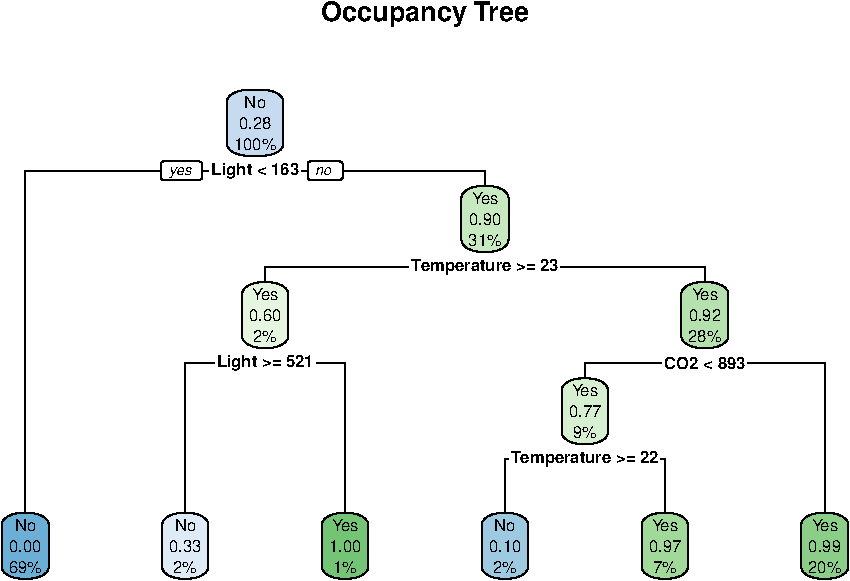
\includegraphics{BSc_CW2_12516369_S_Tariq_files/figure-latex/unnamed-chunk-2-1.pdf}

\begin{Shaded}
\begin{Highlighting}[]
\CommentTok{#interpretation of decision tree}
\KeywordTok{rpart}\NormalTok{(}\DataTypeTok{formula =}\NormalTok{ Occupancy }\OperatorTok{~}\StringTok{ }\NormalTok{.,}\DataTypeTok{data =}\NormalTok{ data_train, }\DataTypeTok{method =} \StringTok{"class"}\NormalTok{)}
\end{Highlighting}
\end{Shaded}

\begin{verbatim}
## n= 2000 
## 
## node), split, n, loss, yval, (yprob)
##       * denotes terminal node
## 
##  1) root 2000 555 No (0.72250000 0.27750000)  
##    2) Light< 162.875 1381   0 No (1.00000000 0.00000000) *
##    3) Light>=162.875 619  64 Yes (0.10339257 0.89660743)  
##      6) Temperature>=22.64167 50  20 Yes (0.40000000 0.60000000)  
##       12) Light>=520.5 30  10 No (0.66666667 0.33333333) *
##       13) Light< 520.5 20   0 Yes (0.00000000 1.00000000) *
##      7) Temperature< 22.64167 569  44 Yes (0.07732865 0.92267135)  
##       14) CO2< 893.125 173  40 Yes (0.23121387 0.76878613)  
##         28) Temperature>=22.21125 40   4 No (0.90000000 0.10000000) *
##         29) Temperature< 22.21125 133   4 Yes (0.03007519 0.96992481) *
##       15) CO2>=893.125 396   4 Yes (0.01010101 0.98989899) *
\end{verbatim}

\hypertarget{c-train-a-random-forests-classifier-and-evaluate-the-predictive-performance-by-reporting-the-accuracy-obtained-on-the-testing-dataset.}{%
\subsubsection{(c) Train a random forests classifier, and evaluate the
predictive performance by reporting the accuracy obtained on the testing
dataset.}\label{c-train-a-random-forests-classifier-and-evaluate-the-predictive-performance-by-reporting-the-accuracy-obtained-on-the-testing-dataset.}}

\begin{Shaded}
\begin{Highlighting}[]
\NormalTok{rf_model <-}\StringTok{ }\KeywordTok{randomForest}\NormalTok{(Occupancy }\OperatorTok{~}\NormalTok{., }\DataTypeTok{data =}\NormalTok{ data_train , }\DataTypeTok{importance =} \OtherTok{TRUE}\NormalTok{)}
\KeywordTok{print}\NormalTok{(rf_model)}
\end{Highlighting}
\end{Shaded}

\begin{verbatim}
## 
## Call:
##  randomForest(formula = Occupancy ~ ., data = data_train, importance = TRUE) 
##                Type of random forest: classification
##                      Number of trees: 500
## No. of variables tried at each split: 2
## 
##         OOB estimate of  error rate: 1.3%
## Confusion matrix:
##       No Yes class.error
## No  1430  15  0.01038062
## Yes   11 544  0.01981982
\end{verbatim}

\begin{Shaded}
\begin{Highlighting}[]
\CommentTok{#evaluate the predictive performance}
\CommentTok{#obtained on the testing dataset}
\NormalTok{rf_pred <-}\StringTok{ }\KeywordTok{predict}\NormalTok{(rf_model,data_test)}
\NormalTok{rf_mat <-}\StringTok{ }\KeywordTok{table}\NormalTok{(rf_pred,data_test}\OperatorTok{$}\NormalTok{Occupancy)}
\KeywordTok{print}\NormalTok{(rf_mat)}
\end{Highlighting}
\end{Shaded}

\begin{verbatim}
##        
## rf_pred  No Yes
##     No  176   6
##     Yes  64  54
\end{verbatim}

\begin{Shaded}
\begin{Highlighting}[]
\CommentTok{#reporting the accuracy}
\NormalTok{accuracy_Test <-}\StringTok{ }\KeywordTok{sum}\NormalTok{(}\KeywordTok{diag}\NormalTok{(rf_mat)) }\OperatorTok{/}\StringTok{ }\KeywordTok{sum}\NormalTok{(rf_mat)}
\KeywordTok{print}\NormalTok{(}\KeywordTok{paste}\NormalTok{(}\StringTok{'Accuracy for test'}\NormalTok{, accuracy_Test))}
\end{Highlighting}
\end{Shaded}

\begin{verbatim}
## [1] "Accuracy for test 0.766666666666667"
\end{verbatim}

\hypertarget{d-output-and-analyse-the-feature-importance-obtained-by-the-random-forests-classifier.}{%
\subsubsection{(d) Output and analyse the feature importance obtained by
the random forests
classifier.}\label{d-output-and-analyse-the-feature-importance-obtained-by-the-random-forests-classifier.}}

\begin{Shaded}
\begin{Highlighting}[]
\CommentTok{#Feature Importance}
\NormalTok{rf_model}\OperatorTok{$}\NormalTok{importance}
\end{Highlighting}
\end{Shaded}

\begin{verbatim}
##                       No        Yes MeanDecreaseAccuracy MeanDecreaseGini
## Temperature   0.03376326 0.07969206           0.04645670        114.56211
## Humidity      0.01344981 0.08876716           0.03439724         29.43368
## Light         0.16822273 0.56439203           0.27797941        403.06189
## CO2           0.03830877 0.24704547           0.09617212        205.31916
## HumidityRatio 0.01623301 0.07209788           0.03177614         47.47406
\end{verbatim}

\hypertarget{svm}{%
\section{3) SVM}\label{svm}}

\hypertarget{to-predict-the-wine-quality-using-the-support-vector-machine-classification-algorithm.}{%
\subsection{To predict the wine quality using the support vector machine
classification
algorithm.}\label{to-predict-the-wine-quality-using-the-support-vector-machine-classification-algorithm.}}

\hypertarget{a-download-the-wine-quality-data-and-use-the-training-dataset-to-conduct-the-grid-search-to-find-the-optimal-hyperparameters-of-svm-by-using-the-linear-kernal.}{%
\subsubsection{(a) Download the wine quality data and use the training
dataset to conduct the grid-search to find the optimal hyperparameters
of svm by using the linear
kernal.}\label{a-download-the-wine-quality-data-and-use-the-training-dataset-to-conduct-the-grid-search-to-find-the-optimal-hyperparameters-of-svm-by-using-the-linear-kernal.}}

\begin{Shaded}
\begin{Highlighting}[]
\KeywordTok{set.seed}\NormalTok{(}\DecValTok{300}\NormalTok{)}
\NormalTok{data_train <-}\StringTok{ }\KeywordTok{read.csv}\NormalTok{(}\DataTypeTok{file=}\StringTok{"WineQuality_training.txt"}\NormalTok{, }\DataTypeTok{header=}\OtherTok{TRUE}\NormalTok{, }\DataTypeTok{sep=}\StringTok{","}\NormalTok{)}
\NormalTok{data_test <-}\StringTok{ }\KeywordTok{read.csv}\NormalTok{(}\DataTypeTok{file=}\StringTok{"WineQuality_testing.txt"}\NormalTok{, }\DataTypeTok{header=}\OtherTok{TRUE}\NormalTok{, }\DataTypeTok{sep=}\StringTok{","}\NormalTok{)}
\CommentTok{#Exploring train DataSet}
\KeywordTok{head}\NormalTok{(data_train)}
\end{Highlighting}
\end{Shaded}

\begin{verbatim}
##   fixed.acidity volatile.acidity citric.acid residual.sugar chlorides
## 1           9.1             0.27        0.45           10.6     0.035
## 2           6.6             0.36        0.29            1.6     0.021
## 3           7.4             0.24        0.36            2.0     0.031
## 4           6.9             0.36        0.34            4.2     0.018
## 5           7.1             0.26        0.49            2.2     0.032
## 6           6.2             0.66        0.48            1.2     0.029
##   free.sulfur.dioxide total.sulfur.dioxide density   pH sulphates alcohol
## 1                  28                  124 0.99700 3.20      0.46    10.4
## 2                  24                   85 0.98965 3.41      0.61    12.4
## 3                  27                  139 0.99055 3.28      0.48    12.5
## 4                  57                  119 0.98980 3.28      0.36    12.7
## 5                  31                  113 0.99030 3.37      0.42    12.9
## 6                  29                   75 0.98920 3.33      0.39    12.8
##   quality
## 1    Good
## 2    Good
## 3    Good
## 4    Good
## 5    Good
## 6    Good
\end{verbatim}

\begin{Shaded}
\begin{Highlighting}[]
\CommentTok{#printing all columns with their data type}
\KeywordTok{str}\NormalTok{(data_train)}
\end{Highlighting}
\end{Shaded}

\begin{verbatim}
## 'data.frame':    3000 obs. of  12 variables:
##  $ fixed.acidity       : num  9.1 6.6 7.4 6.9 7.1 6.2 6.2 6.8 6.7 6.7 ...
##  $ volatile.acidity    : num  0.27 0.36 0.24 0.36 0.26 0.66 0.66 0.26 0.23 0.23 ...
##  $ citric.acid         : num  0.45 0.29 0.36 0.34 0.49 0.48 0.48 0.42 0.31 0.31 ...
##  $ residual.sugar      : num  10.6 1.6 2 4.2 2.2 1.2 1.2 1.7 2.1 2.1 ...
##  $ chlorides           : num  0.035 0.021 0.031 0.018 0.032 0.029 0.029 0.049 0.046 0.046 ...
##  $ free.sulfur.dioxide : num  28 24 27 57 31 29 29 41 30 30 ...
##  $ total.sulfur.dioxide: num  124 85 139 119 113 75 75 122 96 96 ...
##  $ density             : num  0.997 0.99 0.991 0.99 0.99 ...
##  $ pH                  : num  3.2 3.41 3.28 3.28 3.37 3.33 3.33 3.47 3.33 3.33 ...
##  $ sulphates           : num  0.46 0.61 0.48 0.36 0.42 0.39 0.39 0.48 0.64 0.64 ...
##  $ alcohol             : num  10.4 12.4 12.5 12.7 12.9 12.8 12.8 10.5 10.7 10.7 ...
##  $ quality             : Factor w/ 2 levels "Bad","Good": 2 2 2 2 2 2 2 2 2 2 ...
\end{verbatim}

\begin{Shaded}
\begin{Highlighting}[]
\CommentTok{#Checking Null values}
\KeywordTok{any}\NormalTok{(}\KeywordTok{is.na}\NormalTok{(data_train))}
\end{Highlighting}
\end{Shaded}

\begin{verbatim}
## [1] FALSE
\end{verbatim}

\begin{Shaded}
\begin{Highlighting}[]
\KeywordTok{library}\NormalTok{(}\StringTok{"e1071"}\NormalTok{)}
\end{Highlighting}
\end{Shaded}

\begin{verbatim}
## Warning: package 'e1071' was built under R version 3.6.2
\end{verbatim}

\begin{Shaded}
\begin{Highlighting}[]
\NormalTok{model <-}\StringTok{ }\KeywordTok{svm}\NormalTok{(quality }\OperatorTok{~}\NormalTok{., }\DataTypeTok{data =}\NormalTok{ data_train,}\DataTypeTok{kernel =} \StringTok{'linear'}\NormalTok{)}
\KeywordTok{summary}\NormalTok{(model)}
\end{Highlighting}
\end{Shaded}

\begin{verbatim}
## 
## Call:
## svm(formula = quality ~ ., data = data_train, kernel = "linear")
## 
## 
## Parameters:
##    SVM-Type:  C-classification 
##  SVM-Kernel:  linear 
##        cost:  1 
## 
## Number of Support Vectors:  1710
## 
##  ( 855 855 )
## 
## 
## Number of Classes:  2 
## 
## Levels: 
##  Bad Good
\end{verbatim}

\begin{Shaded}
\begin{Highlighting}[]
\CommentTok{#Grid Search using Linear Kernel and finding optimal hyperparameter}
\NormalTok{h_tune <-}\StringTok{ }\KeywordTok{tune}\NormalTok{(svm,}\DataTypeTok{train.x =}\NormalTok{ data_train[}\DecValTok{1}\OperatorTok{:}\DecValTok{11}\NormalTok{] , }\DataTypeTok{train.y =}\NormalTok{ data_train[,}\DecValTok{12}\NormalTok{] ,}
               \DataTypeTok{kernel =} \StringTok{'linear'}\NormalTok{  ,}
               \DataTypeTok{ranges =} \KeywordTok{list}\NormalTok{(}\DataTypeTok{cost =} \KeywordTok{c}\NormalTok{(}\FloatTok{0.01}\NormalTok{, }\FloatTok{0.1}\NormalTok{, }\DecValTok{1}\NormalTok{, }\DecValTok{5}\NormalTok{, }\DecValTok{10}\NormalTok{), }\DataTypeTok{gamma =} \KeywordTok{c}\NormalTok{(}\FloatTok{0.01}\NormalTok{, }\FloatTok{0.03}\NormalTok{, }\FloatTok{0.1}\NormalTok{, }\FloatTok{0.5}\NormalTok{, }\DecValTok{1}\NormalTok{)))}
\KeywordTok{summary}\NormalTok{(h_tune)}
\end{Highlighting}
\end{Shaded}

\begin{verbatim}
## 
## Parameter tuning of 'svm':
## 
## - sampling method: 10-fold cross validation 
## 
## - best parameters:
##  cost gamma
##   0.1  0.01
## 
## - best performance: 0.2376667 
## 
## - Detailed performance results:
##     cost gamma     error dispersion
## 1   0.01  0.01 0.2470000 0.02555314
## 2   0.10  0.01 0.2376667 0.02828645
## 3   1.00  0.01 0.2406667 0.03299083
## 4   5.00  0.01 0.2410000 0.03201273
## 5  10.00  0.01 0.2413333 0.03059896
## 6   0.01  0.03 0.2470000 0.02555314
## 7   0.10  0.03 0.2376667 0.02828645
## 8   1.00  0.03 0.2406667 0.03299083
## 9   5.00  0.03 0.2410000 0.03201273
## 10 10.00  0.03 0.2413333 0.03059896
## 11  0.01  0.10 0.2470000 0.02555314
## 12  0.10  0.10 0.2376667 0.02828645
## 13  1.00  0.10 0.2406667 0.03299083
## 14  5.00  0.10 0.2410000 0.03201273
## 15 10.00  0.10 0.2413333 0.03059896
## 16  0.01  0.50 0.2470000 0.02555314
## 17  0.10  0.50 0.2376667 0.02828645
## 18  1.00  0.50 0.2406667 0.03299083
## 19  5.00  0.50 0.2410000 0.03201273
## 20 10.00  0.50 0.2413333 0.03059896
## 21  0.01  1.00 0.2470000 0.02555314
## 22  0.10  1.00 0.2376667 0.02828645
## 23  1.00  1.00 0.2406667 0.03299083
## 24  5.00  1.00 0.2410000 0.03201273
## 25 10.00  1.00 0.2413333 0.03059896
\end{verbatim}

\hypertarget{b-train-a-svm-classifier-by-using-the-linear-kernal-and-the-corresponding-optimal-hyperparameters-then-make-predictions-on-the-testing-dataset-report-the-predictive-performance.}{%
\subsubsection{(b) Train a svm classifier by using the linear kernal and
the corresponding optimal hyperparameters, then make predictions on the
testing dataset, report the predictive
performance.}\label{b-train-a-svm-classifier-by-using-the-linear-kernal-and-the-corresponding-optimal-hyperparameters-then-make-predictions-on-the-testing-dataset-report-the-predictive-performance.}}

\begin{Shaded}
\begin{Highlighting}[]
\NormalTok{model_lin <-}\StringTok{ }\KeywordTok{svm}\NormalTok{(quality }\OperatorTok{~}\NormalTok{., }\DataTypeTok{data =}\NormalTok{ data_train,}\DataTypeTok{kernel =} \StringTok{'linear'} 
\NormalTok{             , }\DataTypeTok{cost =}\DecValTok{10}\NormalTok{ , }\DataTypeTok{gamma =} \FloatTok{0.01}\NormalTok{ )}

\CommentTok{#make predictions on the testing dataset, }
\CommentTok{#report the predictive performance}

\NormalTok{model_pred <-}\StringTok{ }\KeywordTok{predict}\NormalTok{(model,data_test)}

\CommentTok{#reporting the accuracy}
\NormalTok{svm_mat <-}\StringTok{ }\KeywordTok{table}\NormalTok{(model_pred,data_test}\OperatorTok{$}\NormalTok{quality)}
\KeywordTok{print}\NormalTok{(svm_mat)}
\end{Highlighting}
\end{Shaded}

\begin{verbatim}
##           
## model_pred Bad Good
##       Bad  104   89
##       Good  38  169
\end{verbatim}

\begin{Shaded}
\begin{Highlighting}[]
\NormalTok{accuracy_Test <-}\StringTok{ }\KeywordTok{sum}\NormalTok{(}\KeywordTok{diag}\NormalTok{(svm_mat)) }\OperatorTok{/}\StringTok{ }\KeywordTok{sum}\NormalTok{(svm_mat)}
\KeywordTok{print}\NormalTok{(}\KeywordTok{paste}\NormalTok{(}\StringTok{'Accuracy for test'}\NormalTok{, accuracy_Test))}
\end{Highlighting}
\end{Shaded}

\begin{verbatim}
## [1] "Accuracy for test 0.6825"
\end{verbatim}

\hypertarget{c-conduct-the-grid-search-to-find-the-optimal-hyperparameters-of-svm-by-using-the-rbf-kernal.}{%
\subsubsection{(c) Conduct the grid-search to find the optimal
hyperparameters of svm by using the RBF
kernal.}\label{c-conduct-the-grid-search-to-find-the-optimal-hyperparameters-of-svm-by-using-the-rbf-kernal.}}

\begin{Shaded}
\begin{Highlighting}[]
\CommentTok{#Training SVM using RBF}
\NormalTok{model <-}\StringTok{ }\KeywordTok{svm}\NormalTok{(quality }\OperatorTok{~}\NormalTok{., }\DataTypeTok{data =}\NormalTok{ data_train,  }\DataTypeTok{kernel =} \StringTok{'radial'}\NormalTok{)}

\CommentTok{#Grid Search using RBF Kernel and finding optimal hyperparameter}
\NormalTok{hrbf_tune <-}\StringTok{ }\KeywordTok{tune}\NormalTok{(svm,}\DataTypeTok{train.x =}\NormalTok{ data_train[}\DecValTok{1}\OperatorTok{:}\DecValTok{11}\NormalTok{] , }\DataTypeTok{train.y =}\NormalTok{ data_train[,}\DecValTok{12}\NormalTok{] ,}
               \DataTypeTok{kernel =} \StringTok{'radial'}\NormalTok{  ,}
               \DataTypeTok{ranges =} \KeywordTok{list}\NormalTok{(}\DataTypeTok{cost =} \KeywordTok{c}\NormalTok{(}\FloatTok{0.01}\NormalTok{, }\FloatTok{0.1}\NormalTok{, }\DecValTok{1}\NormalTok{, }\DecValTok{5}\NormalTok{, }\DecValTok{10}\NormalTok{), }\DataTypeTok{gamma =} \KeywordTok{c}\NormalTok{(}\FloatTok{0.01}\NormalTok{, }\FloatTok{0.03}\NormalTok{, }\FloatTok{0.1}\NormalTok{, }\FloatTok{0.5}\NormalTok{, }\DecValTok{1}\NormalTok{)))}
\KeywordTok{summary}\NormalTok{(hrbf_tune)}
\end{Highlighting}
\end{Shaded}

\begin{verbatim}
## 
## Parameter tuning of 'svm':
## 
## - sampling method: 10-fold cross validation 
## 
## - best parameters:
##  cost gamma
##     5   0.5
## 
## - best performance: 0.159 
## 
## - Detailed performance results:
##     cost gamma     error dispersion
## 1   0.01  0.01 0.2886667 0.02079886
## 2   0.10  0.01 0.2520000 0.01853925
## 3   1.00  0.01 0.2363333 0.01842234
## 4   5.00  0.01 0.2076667 0.01785055
## 5  10.00  0.01 0.2070000 0.01702939
## 6   0.01  0.03 0.2673333 0.01698220
## 7   0.10  0.03 0.2400000 0.02479546
## 8   1.00  0.03 0.2063333 0.02151371
## 9   5.00  0.03 0.1956667 0.02024846
## 10 10.00  0.03 0.1966667 0.01706921
## 11  0.01  0.10 0.2676667 0.02378141
## 12  0.10  0.10 0.2073333 0.01824389
## 13  1.00  0.10 0.1930000 0.01828782
## 14  5.00  0.10 0.1806667 0.01553967
## 15 10.00  0.10 0.1750000 0.01649916
## 16  0.01  0.50 0.5126667 0.07542145
## 17  0.10  0.50 0.2323333 0.02336242
## 18  1.00  0.50 0.1656667 0.01625795
## 19  5.00  0.50 0.1590000 0.01735967
## 20 10.00  0.50 0.1613333 0.02440401
## 21  0.01  1.00 0.5153333 0.06737036
## 22  0.10  1.00 0.2706667 0.05941692
## 23  1.00  1.00 0.1673333 0.01748368
## 24  5.00  1.00 0.1613333 0.01813529
## 25 10.00  1.00 0.1623333 0.01918397
\end{verbatim}

\begin{Shaded}
\begin{Highlighting}[]
\NormalTok{model_rbf <-}\StringTok{ }\KeywordTok{svm}\NormalTok{(quality }\OperatorTok{~}\NormalTok{., }\DataTypeTok{data =}\NormalTok{ data_train,}\DataTypeTok{kernel =} \StringTok{'radial'} 
\NormalTok{             , }\DataTypeTok{cost =}\DecValTok{5}\NormalTok{ , }\DataTypeTok{gamma =} \FloatTok{0.5}\NormalTok{ ,}\DataTypeTok{decision.values =} \OtherTok{TRUE}\NormalTok{,}\DataTypeTok{probability =} \OtherTok{TRUE}\NormalTok{)}

\NormalTok{model_predrbf <-}\StringTok{ }\KeywordTok{predict}\NormalTok{(model_rbf,data_test)}

\KeywordTok{print}\NormalTok{(model_predrbf)}
\end{Highlighting}
\end{Shaded}

\begin{verbatim}
##    1    2    3    4    5    6    7    8    9   10   11   12   13   14   15 
## Good Good  Bad  Bad Good Good Good  Bad Good Good Good Good  Bad Good  Bad 
##   16   17   18   19   20   21   22   23   24   25   26   27   28   29   30 
## Good Good Good Good  Bad Good Good Good Good Good Good Good  Bad  Bad  Bad 
##   31   32   33   34   35   36   37   38   39   40   41   42   43   44   45 
##  Bad Good  Bad  Bad Good Good Good Good Good Good Good Good  Bad  Bad  Bad 
##   46   47   48   49   50   51   52   53   54   55   56   57   58   59   60 
##  Bad  Bad  Bad Good  Bad  Bad  Bad  Bad Good Good  Bad  Bad Good Good Good 
##   61   62   63   64   65   66   67   68   69   70   71   72   73   74   75 
## Good Good Good Good Good Good Good Good Good  Bad Good Good Good Good Good 
##   76   77   78   79   80   81   82   83   84   85   86   87   88   89   90 
## Good Good Good  Bad  Bad Good  Bad  Bad Good Good Good Good Good  Bad  Bad 
##   91   92   93   94   95   96   97   98   99  100  101  102  103  104  105 
## Good  Bad Good  Bad Good  Bad  Bad  Bad Good Good  Bad Good Good  Bad  Bad 
##  106  107  108  109  110  111  112  113  114  115  116  117  118  119  120 
##  Bad Good Good  Bad Good Good  Bad Good Good  Bad Good  Bad Good Good  Bad 
##  121  122  123  124  125  126  127  128  129  130  131  132  133  134  135 
## Good Good Good Good Good Good  Bad Good  Bad  Bad Good  Bad Good Good  Bad 
##  136  137  138  139  140  141  142  143  144  145  146  147  148  149  150 
##  Bad  Bad  Bad  Bad Good  Bad  Bad  Bad  Bad Good Good  Bad Good Good Good 
##  151  152  153  154  155  156  157  158  159  160  161  162  163  164  165 
## Good  Bad Good  Bad  Bad  Bad Good  Bad  Bad Good Good  Bad  Bad Good Good 
##  166  167  168  169  170  171  172  173  174  175  176  177  178  179  180 
## Good  Bad Good Good Good Good Good Good Good  Bad Good  Bad  Bad Good Good 
##  181  182  183  184  185  186  187  188  189  190  191  192  193  194  195 
##  Bad Good  Bad  Bad Good Good  Bad  Bad  Bad  Bad  Bad  Bad Good  Bad  Bad 
##  196  197  198  199  200  201  202  203  204  205  206  207  208  209  210 
##  Bad Good Good  Bad  Bad  Bad Good  Bad  Bad  Bad Good  Bad  Bad Good  Bad 
##  211  212  213  214  215  216  217  218  219  220  221  222  223  224  225 
## Good Good Good Good Good Good Good Good  Bad  Bad Good Good Good Good  Bad 
##  226  227  228  229  230  231  232  233  234  235  236  237  238  239  240 
## Good  Bad Good  Bad  Bad Good Good Good  Bad Good  Bad Good Good Good Good 
##  241  242  243  244  245  246  247  248  249  250  251  252  253  254  255 
##  Bad Good  Bad Good Good Good Good  Bad  Bad  Bad  Bad  Bad  Bad Good Good 
##  256  257  258  259  260  261  262  263  264  265  266  267  268  269  270 
## Good Good Good  Bad  Bad  Bad  Bad Good  Bad  Bad  Bad  Bad  Bad  Bad  Bad 
##  271  272  273  274  275  276  277  278  279  280  281  282  283  284  285 
##  Bad  Bad  Bad  Bad  Bad  Bad  Bad  Bad  Bad  Bad  Bad  Bad  Bad  Bad  Bad 
##  286  287  288  289  290  291  292  293  294  295  296  297  298  299  300 
##  Bad  Bad Good  Bad  Bad  Bad  Bad  Bad  Bad  Bad Good Good  Bad  Bad Good 
##  301  302  303  304  305  306  307  308  309  310  311  312  313  314  315 
## Good  Bad  Bad Good  Bad  Bad  Bad  Bad  Bad  Bad  Bad  Bad Good  Bad  Bad 
##  316  317  318  319  320  321  322  323  324  325  326  327  328  329  330 
## Good  Bad Good  Bad  Bad  Bad  Bad Good Good  Bad  Bad  Bad  Bad  Bad  Bad 
##  331  332  333  334  335  336  337  338  339  340  341  342  343  344  345 
## Good Good  Bad  Bad Good  Bad Good  Bad  Bad Good Good  Bad  Bad  Bad  Bad 
##  346  347  348  349  350  351  352  353  354  355  356  357  358  359  360 
##  Bad  Bad  Bad Good Good  Bad  Bad  Bad  Bad  Bad  Bad  Bad  Bad  Bad  Bad 
##  361  362  363  364  365  366  367  368  369  370  371  372  373  374  375 
## Good  Bad  Bad  Bad Good Good  Bad Good  Bad Good  Bad  Bad  Bad  Bad  Bad 
##  376  377  378  379  380  381  382  383  384  385  386  387  388  389  390 
##  Bad Good  Bad Good  Bad  Bad  Bad  Bad  Bad  Bad  Bad  Bad  Bad  Bad  Bad 
##  391  392  393  394  395  396  397  398  399  400 
##  Bad  Bad  Bad  Bad  Bad Good Good  Bad  Bad  Bad 
## Levels: Bad Good
\end{verbatim}

\begin{Shaded}
\begin{Highlighting}[]
\KeywordTok{summary}\NormalTok{(model_predrbf)}
\end{Highlighting}
\end{Shaded}

\begin{verbatim}
##  Bad Good 
##  221  179
\end{verbatim}

\hypertarget{d-train-a-svm-classifier-by-using-the-rbf-kernal-and-the-corresponding-optimal-hyperparameters-then-make-predictions-on-the-testing-dataset-report-the-predictive-performance.}{%
\subsubsection{(d) Train a svm classifier by using the RBF kernal and
the corresponding optimal hyperparameters, then make predictions on the
testing dataset, report the predictive
performance.}\label{d-train-a-svm-classifier-by-using-the-rbf-kernal-and-the-corresponding-optimal-hyperparameters-then-make-predictions-on-the-testing-dataset-report-the-predictive-performance.}}

\begin{Shaded}
\begin{Highlighting}[]
\NormalTok{svm.rbf_mat <-}\StringTok{ }\KeywordTok{table}\NormalTok{(model_predrbf,data_test}\OperatorTok{$}\NormalTok{quality)}
\KeywordTok{print}\NormalTok{(svm.rbf_mat)}
\end{Highlighting}
\end{Shaded}

\begin{verbatim}
##              
## model_predrbf Bad Good
##          Bad  113  108
##          Good  29  150
\end{verbatim}

\begin{Shaded}
\begin{Highlighting}[]
\NormalTok{accuracy_Test <-}\StringTok{ }\KeywordTok{sum}\NormalTok{(}\KeywordTok{diag}\NormalTok{(svm.rbf_mat)) }\OperatorTok{/}\StringTok{ }\KeywordTok{sum}\NormalTok{(svm.rbf_mat)}
\KeywordTok{print}\NormalTok{(}\KeywordTok{paste}\NormalTok{(}\StringTok{'Accuracy for test'}\NormalTok{, accuracy_Test))}
\end{Highlighting}
\end{Shaded}

\begin{verbatim}
## [1] "Accuracy for test 0.6575"
\end{verbatim}

\hypertarget{e-conduct-the-roc-curve-analysis-to-compare-the-predictive-performance-of-svm-classifiers-trained-by-using-the-linear-and-rbf-kernels-respectively.}{%
\subsubsection{(e) Conduct the ROC curve analysis to compare the
predictive performance of svm classifiers trained by using the linear
and RBF kernels
respectively.}\label{e-conduct-the-roc-curve-analysis-to-compare-the-predictive-performance-of-svm-classifiers-trained-by-using-the-linear-and-rbf-kernels-respectively.}}

\hypertarget{hint-given-a-pre-defined-hyperparameter-space---c-0.01-0.1-1-5-10-and-ux3b3-0.01-0.03-0.1-0.5-1.}{%
\paragraph{Hint: Given a pre-defined hyperparameter space - C: {[}0.01,
0.1, 1, 5, 10{]}, and γ: {[}0.01, 0.03, 0.1, 0.5,
1{]}.}\label{hint-given-a-pre-defined-hyperparameter-space---c-0.01-0.1-1-5-10-and-ux3b3-0.01-0.03-0.1-0.5-1.}}

\begin{Shaded}
\begin{Highlighting}[]
\KeywordTok{library}\NormalTok{(}\StringTok{"ROSE"}\NormalTok{)}
\end{Highlighting}
\end{Shaded}

\begin{verbatim}
## Warning: package 'ROSE' was built under R version 3.6.2
\end{verbatim}

\begin{verbatim}
## Loaded ROSE 0.0-3
\end{verbatim}

\begin{Shaded}
\begin{Highlighting}[]
\NormalTok{rbf_pred <-}\StringTok{ }\KeywordTok{predict}\NormalTok{(model_rbf,data_test)}
\NormalTok{lin_pred <-}\StringTok{ }\KeywordTok{predict}\NormalTok{(model_lin,data_test)}

\NormalTok{rbf_pred <-}\StringTok{ }\KeywordTok{prediction}\NormalTok{(}\KeywordTok{as.numeric}\NormalTok{(rbf_pred) , }\KeywordTok{as.numeric}\NormalTok{(data_test}\OperatorTok{$}\NormalTok{quality))}
\NormalTok{roc <-}\StringTok{ }\KeywordTok{performance}\NormalTok{(rbf_pred,}\StringTok{'tpr'}\NormalTok{,}\StringTok{'fpr'}\NormalTok{)}
\KeywordTok{plot}\NormalTok{(roc , }\DataTypeTok{main =} \StringTok{"ROC for RBF Kernel"}\NormalTok{,}\DataTypeTok{col =} \StringTok{'red'}\NormalTok{)}
\KeywordTok{abline}\NormalTok{(}\DataTypeTok{a=}\DecValTok{0}\NormalTok{, }\DataTypeTok{b=}\DecValTok{1}\NormalTok{,}\DataTypeTok{col =} \StringTok{'blue'}\NormalTok{)}
\end{Highlighting}
\end{Shaded}

\includegraphics{BSc_CW2_12516369_S_Tariq_files/figure-latex/unnamed-chunk-9-1.pdf}

\begin{Shaded}
\begin{Highlighting}[]
\NormalTok{lin_pred <-}\StringTok{ }\KeywordTok{prediction}\NormalTok{(}\KeywordTok{as.numeric}\NormalTok{(lin_pred) , }\KeywordTok{as.numeric}\NormalTok{(data_test}\OperatorTok{$}\NormalTok{quality))}
\NormalTok{roc <-}\StringTok{ }\KeywordTok{performance}\NormalTok{(lin_pred,}\StringTok{'tpr'}\NormalTok{,}\StringTok{'fpr'}\NormalTok{)}
\KeywordTok{plot}\NormalTok{(roc , }\DataTypeTok{main =} \StringTok{"ROC for Linear Kernel"}\NormalTok{,}\DataTypeTok{col =} \StringTok{'red'}\NormalTok{)}
\KeywordTok{abline}\NormalTok{(}\DataTypeTok{a=}\DecValTok{0}\NormalTok{, }\DataTypeTok{b=}\DecValTok{1}\NormalTok{,}\DataTypeTok{col =} \StringTok{'blue'}\NormalTok{)}
\end{Highlighting}
\end{Shaded}

\includegraphics{BSc_CW2_12516369_S_Tariq_files/figure-latex/unnamed-chunk-9-2.pdf}

\hypertarget{hierarchical-clustering}{%
\section{4) Hierarchical Clustering}\label{hierarchical-clustering}}

\hypertarget{consider-the-usarrests-data.-we-will-now-perform-hierarchical-clustering-on-the-states.}{%
\subsection{Consider the USArrests data. We will now perform
hierarchical clustering on the
states.}\label{consider-the-usarrests-data.-we-will-now-perform-hierarchical-clustering-on-the-states.}}

\hypertarget{a-using-hierarchical-clustering-with-complete-linkage-and-euclidean-distance-cluster-the-states.}{%
\subsubsection{(a) Using hierarchical clustering with complete linkage
and Euclidean distance, cluster the
states.}\label{a-using-hierarchical-clustering-with-complete-linkage-and-euclidean-distance-cluster-the-states.}}

\begin{Shaded}
\begin{Highlighting}[]
\KeywordTok{data}\NormalTok{(}\StringTok{"USArrests"}\NormalTok{)}
\NormalTok{data_sets<-USArrests }
\KeywordTok{head}\NormalTok{(data_sets)}
\end{Highlighting}
\end{Shaded}

\begin{verbatim}
##            Murder Assault UrbanPop Rape
## Alabama      13.2     236       58 21.2
## Alaska       10.0     263       48 44.5
## Arizona       8.1     294       80 31.0
## Arkansas      8.8     190       50 19.5
## California    9.0     276       91 40.6
## Colorado      7.9     204       78 38.7
\end{verbatim}

\begin{Shaded}
\begin{Highlighting}[]
\KeywordTok{str}\NormalTok{(data_sets)}
\end{Highlighting}
\end{Shaded}

\begin{verbatim}
## 'data.frame':    50 obs. of  4 variables:
##  $ Murder  : num  13.2 10 8.1 8.8 9 7.9 3.3 5.9 15.4 17.4 ...
##  $ Assault : int  236 263 294 190 276 204 110 238 335 211 ...
##  $ UrbanPop: int  58 48 80 50 91 78 77 72 80 60 ...
##  $ Rape    : num  21.2 44.5 31 19.5 40.6 38.7 11.1 15.8 31.9 25.8 ...
\end{verbatim}

\begin{Shaded}
\begin{Highlighting}[]
\KeywordTok{any}\NormalTok{(}\KeywordTok{is.na}\NormalTok{(data_sets))}
\end{Highlighting}
\end{Shaded}

\begin{verbatim}
## [1] FALSE
\end{verbatim}

\begin{Shaded}
\begin{Highlighting}[]
\KeywordTok{summary}\NormalTok{(data_sets)}
\end{Highlighting}
\end{Shaded}

\begin{verbatim}
##      Murder          Assault         UrbanPop          Rape      
##  Min.   : 0.800   Min.   : 45.0   Min.   :32.00   Min.   : 7.30  
##  1st Qu.: 4.075   1st Qu.:109.0   1st Qu.:54.50   1st Qu.:15.07  
##  Median : 7.250   Median :159.0   Median :66.00   Median :20.10  
##  Mean   : 7.788   Mean   :170.8   Mean   :65.54   Mean   :21.23  
##  3rd Qu.:11.250   3rd Qu.:249.0   3rd Qu.:77.75   3rd Qu.:26.18  
##  Max.   :17.400   Max.   :337.0   Max.   :91.00   Max.   :46.00
\end{verbatim}

\begin{Shaded}
\begin{Highlighting}[]
\NormalTok{data<-}\KeywordTok{dist}\NormalTok{(data_sets, }\DataTypeTok{method =} \StringTok{'euclidean'}\NormalTok{)}
\CommentTok{#hierarchical clustering}
\NormalTok{hiera_data<-}\KeywordTok{hclust}\NormalTok{(data)}
\CommentTok{#cluster the states}
\KeywordTok{plot}\NormalTok{(hiera_data)}
\end{Highlighting}
\end{Shaded}

\includegraphics{BSc_CW2_12516369_S_Tariq_files/figure-latex/unnamed-chunk-10-1.pdf}

\hypertarget{b-cut-the-dendrogram-at-a-height-that-results-in-three-distinct-clusters.-which-states-belong-to-which-clusters}{%
\subsubsection{(b) Cut the dendrogram at a height that results in three
distinct clusters. Which states belong to which
clusters?}\label{b-cut-the-dendrogram-at-a-height-that-results-in-three-distinct-clusters.-which-states-belong-to-which-clusters}}

\begin{Shaded}
\begin{Highlighting}[]
\NormalTok{clust_avg <-}\StringTok{ }\KeywordTok{hclust}\NormalTok{(data, }\DataTypeTok{method =} \StringTok{'average'}\NormalTok{)}
\KeywordTok{plot}\NormalTok{(clust_avg)}
\NormalTok{cut_avg <-}\StringTok{ }\KeywordTok{cutree}\NormalTok{(clust_avg, }\DataTypeTok{k =} \DecValTok{3}\NormalTok{)}
\KeywordTok{plot}\NormalTok{(clust_avg)}
\KeywordTok{rect.hclust}\NormalTok{(clust_avg , }\DataTypeTok{k =} \DecValTok{3}\NormalTok{, }\DataTypeTok{border =} \DecValTok{2}\OperatorTok{:}\DecValTok{6}\NormalTok{)}
\KeywordTok{abline}\NormalTok{(}\DataTypeTok{h =} \DecValTok{3}\NormalTok{, }\DataTypeTok{col =} \StringTok{'blue'}\NormalTok{)}
\end{Highlighting}
\end{Shaded}

\includegraphics{BSc_CW2_12516369_S_Tariq_files/figure-latex/unnamed-chunk-11-1.pdf}

\hypertarget{c-hierarchically-cluster-the-states-using-complete-linkage-and-euclidean-distance-after-scaling-the-variables-to-have-standard-deviation-one.}{%
\subsubsection{(c) Hierarchically cluster the states using complete
linkage and Euclidean distance, after scaling the variables to have
standard deviation
one.}\label{c-hierarchically-cluster-the-states-using-complete-linkage-and-euclidean-distance-after-scaling-the-variables-to-have-standard-deviation-one.}}

\begin{Shaded}
\begin{Highlighting}[]
\NormalTok{data_sets <-}\StringTok{ }\KeywordTok{as.data.frame}\NormalTok{(}\KeywordTok{scale}\NormalTok{(data_sets))}

\NormalTok{data<-}\KeywordTok{dist}\NormalTok{(data_sets, }\DataTypeTok{method =} \StringTok{'euclidean'}\NormalTok{)}
\CommentTok{#hierarchical clustering}
\NormalTok{hiera_data<-}\KeywordTok{hclust}\NormalTok{(data)}
\CommentTok{#cluster the states}
\KeywordTok{plot}\NormalTok{(hiera_data)}
\end{Highlighting}
\end{Shaded}

\includegraphics{BSc_CW2_12516369_S_Tariq_files/figure-latex/unnamed-chunk-12-1.pdf}

\hypertarget{d-what-effect-does-scaling-the-variables-have-on-the-hierarchical-clustering-obtained-in-your-opinion-should-the-variables-be-scaled-before-the-inter-observation-dissimilarities-are-computed-provide-a-justification-for-your-answer.}{%
\subsubsection{(d) What effect does scaling the variables have on the
hierarchical clustering obtained? In your opinion, should the variables
be scaled before the inter-observation dissimilarities are computed?
Provide a justification for your
answer.}\label{d-what-effect-does-scaling-the-variables-have-on-the-hierarchical-clustering-obtained-in-your-opinion-should-the-variables-be-scaled-before-the-inter-observation-dissimilarities-are-computed-provide-a-justification-for-your-answer.}}

In scaling we are transforming numerical values to get specific helpful
properties In scaling we are changing the range of data as we can see
earlier the range/height was 0-300 and after scaling it shrinks to
0-6.We should have scaled the data before because whenever we have
parameters/Features that differ from each other in terms of range of
values then you have to normalise the data so that the difference in
these range of values does not affect your outcome.


\end{document}
